\section{Phương pháp đề xuất}

\subsection{Kiến trúc tổng thể}

Hệ thống được thiết kế theo kiến trúc ba tầng với cơ chế tải mô hình lười biếng (lazy loading) và đồng bộ hóa đa luồng:

\begin{itemize}[leftmargin=*,nosep]
  \item \textbf{Tầng AI suy luận (Python/OpenCV):} Gồm 7 mô hình AI được tải vào bộ nhớ thông qua cơ chế {\tt \_load\_once()} với khóa đồng bộ (threading.Lock) để đảm bảo an toàn đa luồng. Mỗi mô hình chỉ được khởi tạo một lần duy nhất khi có yêu cầu đầu tiên, giảm thời gian khởi động và tiết kiệm bộ nhớ. Các mô hình bao gồm: dlib face detector, dlib shape predictor (68 điểm), YOLOv8n (COCO), YOLOv8 day\_an\_toan, YOLOv8 bien\_bao, YOLOv8 lech\_lan, YOLOv8 vat\_can, MediaPipe Hands/Pose.
  \item \textbf{Tầng backend Flask API:} Cung cấp REST API, WebSocket cho truyền thông thời gian thực và MQTT cho kết nối IoT (ESP32). Hàng đợi cảnh báo AI {\tt ai\_alerts\_queue} duy trì tối đa 50 sự kiện gần nhất với cơ chế đồng bộ riêng.
  \item \textbf{Tầng giao diện web:} Dashboard giám sát thời gian thực, hiển thị video stream, thống kê cảnh báo và lịch sử vi phạm.
\end{itemize}

Cơ chế tải mô hình được thiết kế an toàn đa luồng thông qua mẫu thiết kế double-checked locking:

\begin{algorithm}[!ht]
\caption{Cơ chế tải mô hình lười biếng an toàn đa luồng}
\fontsize{8}{10}\selectfont
\begin{algorithmic}[1]
\Procedure{load\_once}{name, factory}
    \State value $\gets$ globals[name]
    \If{value == None}
        \State model\_lock.acquire()
        \State value $\gets$ globals[name]
        \If{value == None}
            \State value $\gets$ factory()
            \State globals[name] $\gets$ value
        \EndIf
        \State model\_lock.release()
    \EndIf
    \State \Return value
\EndProcedure
\end{algorithmic}
\end{algorithm}

Mỗi module AI trong pipeline được trang bị cơ chế bật/tắt (toggle) độc lập thông qua biến {\tt warning\_states}, cho phép linh hoạt cấu hình module theo nhu cầu giám sát. Thời gian suy luận của từng module được đo lường và lưu vào {\tt timing\_stats} để đánh giá hiệu năng chi tiết.

\subsection{Module phát hiện hành vi tài xế}

\subsubsection{Phát hiện nhắm mắt và buồn ngủ}
Module sử dụng bộ phát hiện khuôn mặt dlib và bộ dự đoán điểm mốc 68 điểm \cite{king2009}. Chỉ số EAR được tính cho từng mắt từ 6 điểm mốc (index 36--41 cho mắt trái, 42--47 cho mắt phải):

\begin{equation}
EAR = \frac{\|p_2 - p_6\| + \|p_3 - p_5\|}{2\|p_1 - p_4\|}
\label{eq:ear}
\end{equation}
Ngưỡng phát hiện nhắm mắt: $EAR < 0.30$ trong thời gian tối thiểu 2 giây liên tục.
\subsubsection{Phát hiện ngáp}
Phát hiện ngáp dựa trên khoảng cách giữa môi trên và môi dưới từ các điểm mốc khuôn mặt:

\begin{equation}
MAR = \frac{1}{|bottom|} \sum_{i \in bottom} y_i - \frac{1}{|top|} \sum_{j \in top} y_j
\label{eq:mar}
\end{equation}

Trong đó $bottom = \{56,57,58,65,66\}$, $top = \{50,51,52,61,62\}$.
Ngưỡng phát hiện: $MAR > 25$ pixel trong 15 khung hình liên tiếp (~0,75 giây).

\subsubsection{Ước lượng tư thế đầu}

Sử dụng thuật toán solvePnP của OpenCV với mô hình khuôn mặt 3D và sáu điểm mốc (mũi, cằm, khóe mắt, khóe miệng). Phương trình chiếu:

\begin{equation}
s \cdot \begin{bmatrix} u \\ v \\ 1 \end{bmatrix} = 
K \cdot [R \;|\; t] \cdot \begin{bmatrix} X \\ Y \\ Z \\ 1 \end{bmatrix}
\label{eq:pnp}
\end{equation}

Kết quả trả về ba góc Euler. Ngưỡng cảnh báo: $|yaw| > 40^\circ$ hoặc $pitch > 35^\circ$.

\subsubsection{Phát hiện sử dụng điện thoại}

Mô hình YOLOv8n \cite{jocher2023} được fine-tuning trên 8.500 ảnh cabin kết hợp pretrained COCO (80 lớp) với freezing layers. Kết quả huấn luyện (Bảng~\ref{tab:yolo_training}) đạt mAP@50 = 0,975 và mAP@50--95 = 0,748 sau 100 epoch. Hình~\ref{fig:training_curves} cho thấy các chỉ số hội tụ ổn định từ epoch 50. Ma trận nhầm lẫn (Hình~\ref{fig:confusion_matrix}) xác nhận độ chính xác phân loại cao giữa lớp ``cell phone'' và nền. Hệ thống xác định hành vi sử dụng điện thoại khi độ tin cậy dự đoán vượt ngưỡng 0,5.

\begin{figure}[H]
\centering

\includegraphics[width=\columnwidth]{phone_results.png}
\caption{Đường cong huấn luyện mô hình phát hiện điện thoại}
\label{fig:training_curves}
\end{figure}

\begin{figure}[H]
\centering

\includegraphics[width=\columnwidth]{phone_confusion.png}
\caption{Ma trận nhầm lẫn của mô hình phát hiện điện thoại}
\label{fig:confusion_matrix}
\end{figure}

\subsubsection{Phát hiện dây an toàn}

Module sử dụng YOLOv8 được huấn luyện tùy chỉnh (trọng số {\tt day\_an\_toan.pt}) trên tập dữ liệu 1.200 ảnh thu thập từ nhiều góc nhìn trong cabin, áp dụng transfer learning với fine-tuning. Kết quả (Bảng~\ref{tab:yolo_training}) đạt mAP@50 = 0,753 và mAP@50--95 = 0,354 sau 50 epoch. Độ chính xác thấp hơn so với mô hình điện thoại do kích thước tập dữ liệu nhỏ hơn và sự đa dạng về tư thế, góc nhìn của dây an toàn.

\begin{figure}[H]
\centering
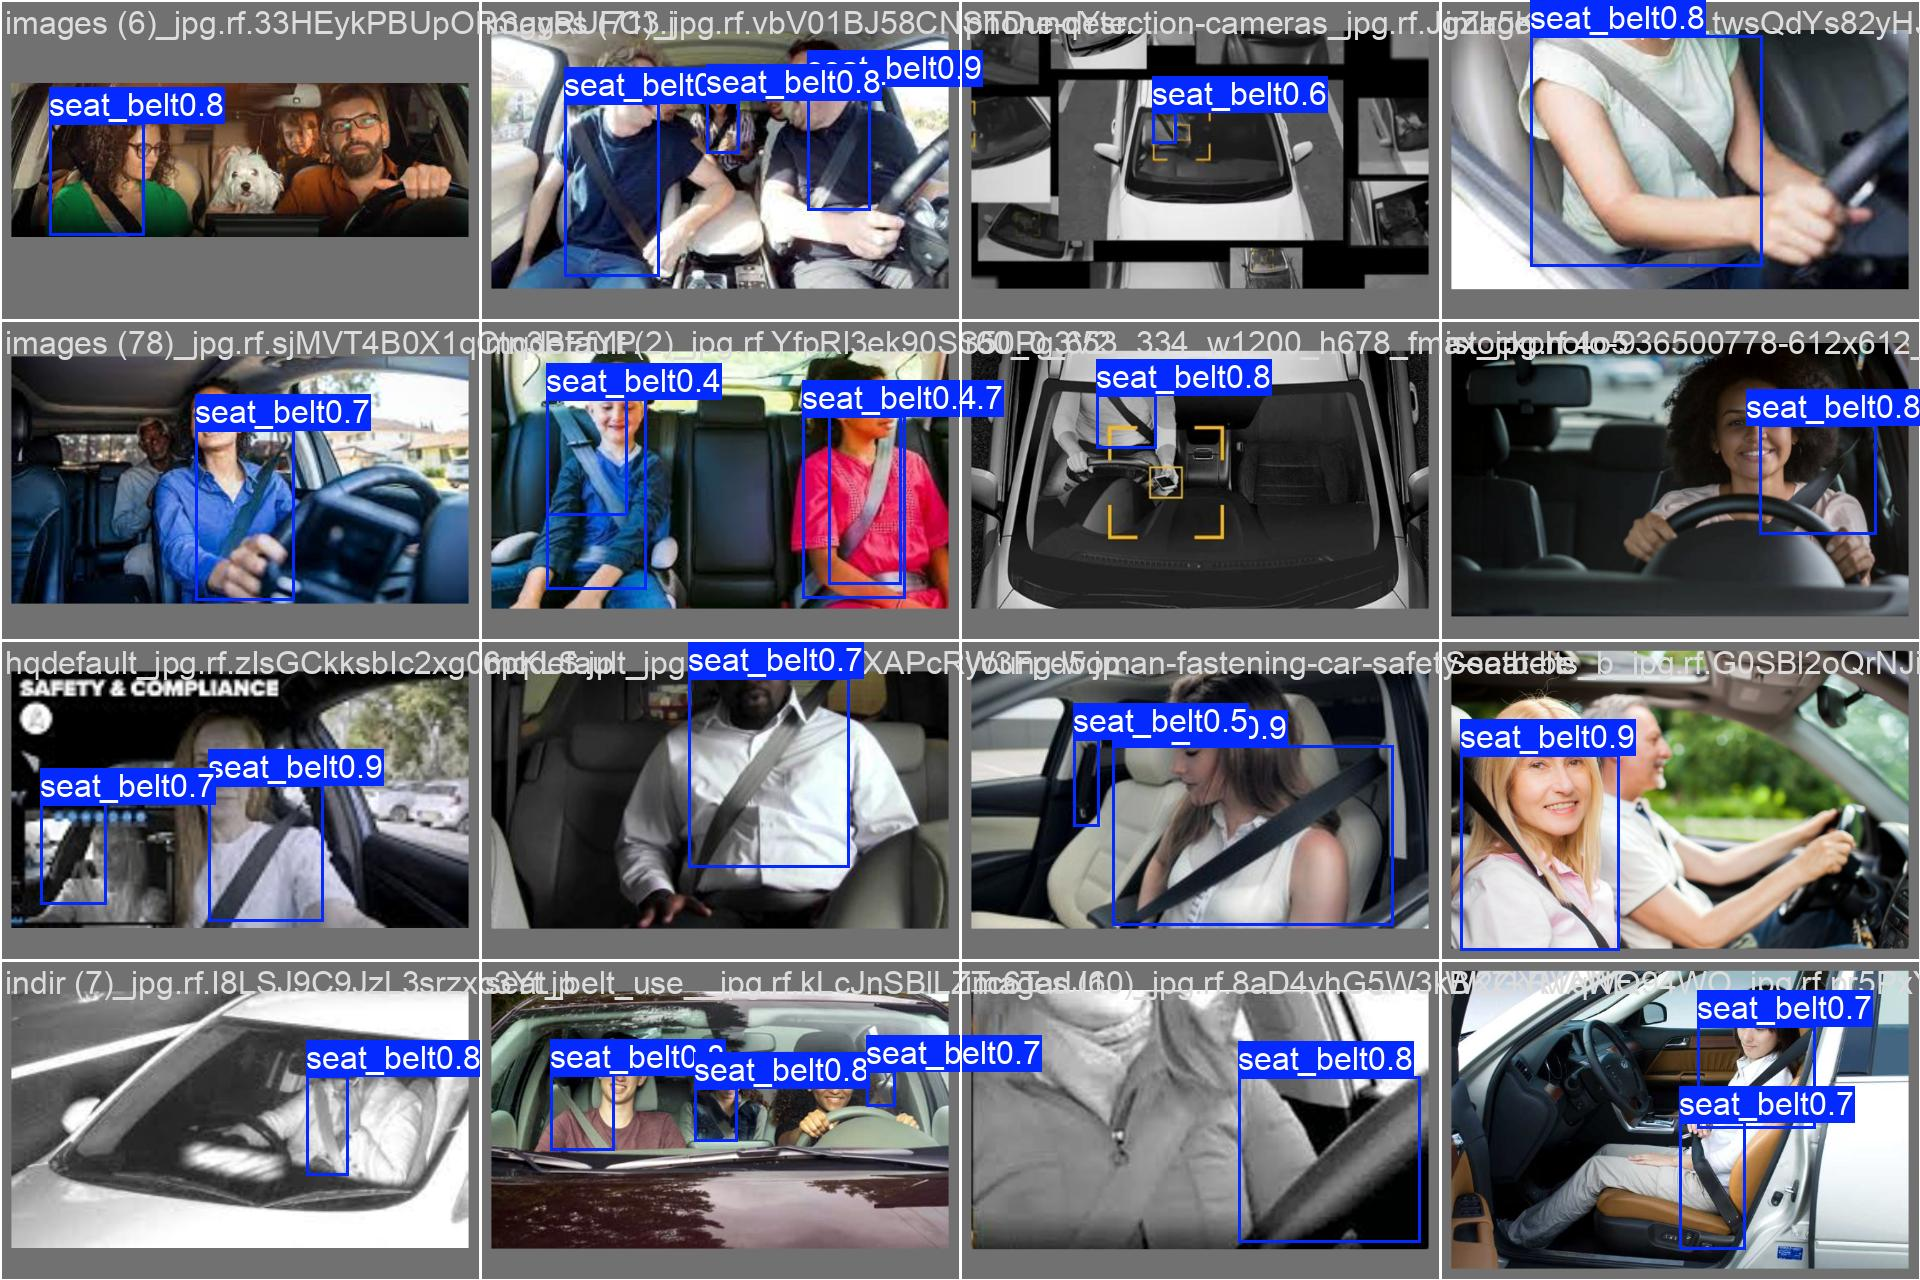
\includegraphics[width=\columnwidth]{images/seatbelt_detection.jpg}
\caption{Kết quả phát hiện dây an toàn trên ảnh thực tế}
\label{fig:detection_examples}
\end{figure}

\begin{table}[H]
\centering
\caption{Kết quả huấn luyện các mô hình YOLO}
\fontsize{7}{8.5}\selectfont
\setlength{\tabcolsep}{2.5pt}
\resizebox{\columnwidth}{!}{%
\begin{tabular}{lcccc}
\toprule
Mô hình & Dữ liệu & Số ảnh & mAP@50 & mAP@50--95 \\
\midrule
CellPhone-YOLOv8n & COCO + In-Cabin Real & 8.500 & 0,975 & 0,748 \\
Seatbelt-YOLOv8 & Custom In-Cabin & 1.200 & 0,753 & 0,354 \\
\bottomrule
\end{tabular}
}
\label{tab:yolo_training}
\end{table}

\subsubsection{Theo dõi tay lái}

Module sử dụng MediaPipe Hands \cite{lugaresi2019} (21 landmarks, detection confidence 0,5) và MediaPipe Pose (33 landmarks) qua lớp {\tt HandAndArmTracking}. Bộ phân loại nắm tay (fist classifier) kiểm tra 4 ngón (trỏ, giữa, áp út, út) dựa trên vị trí đầu ngón so với khớp ngón:

\begin{equation}
FistScore = \sum_{k \in \{8,12,16,20\}} [\,landmark_k.y > landmark_{k-2}.y\,]
\label{eq:fist}
\end{equation}

Các chỉ số: 8/12/16/20 (đầu ngón), 6/10/14/18 (khớp ngón). Ngón cái (4/3) được loại trừ. Nắm vô lăng được xác định khi $FistScore \geq 3$. Cảnh báo kích hoạt nếu không phát hiện nắm trong 3 giây liên tục, khoảng cách giữa các cảnh báo tối thiểu 5 giây.

\subsection{Pipeline xử lý AI}

Pipeline tổng thể hoạt động theo cơ chế xử lý tuần tự kết hợp đo lường hiệu năng từng module. Mỗi module có thể được bật/tắt độc lập thông qua biến {\tt warning\_states}. Thời gian suy luận của từng module được ghi nhận vào {\tt timing\_stats} để phục vụ đánh giá. Pipeline tổng thể được mô tả trong Thuật toán~\ref{alg:pipeline}.

\begin{algorithm}[!ht]
\caption{Pipeline suy luận AI tổng thể}
\label{alg:pipeline}
\fontsize{8}{10}\selectfont
\begin{algorithmic}[1]
\State \textbf{Input:} Video stream từ camera tài xế
\State \textbf{Output:} Frame đã annotate + cảnh báo
\State Khởi tạo toàn bộ mô hình (dlib, YOLOv8, MediaPipe)
\While{đang giám sát}
    \State frame $\gets$ cap.read()
    \State gray $\gets$ cv2.cvtColor(frame, cv2.COLOR\_BGR2GRAY)
    \If{module mắt được bật}
        \State faces $\gets$ face\_detector(gray)
        \State shape $\gets$ landmark\_predictor(gray, face)
        \State ear $\gets$ eye\_aspect\_ratio(shape)
        \If{ear $<$ EAR\_THRESHOLD \textbf{và} duration $>$ 2s}
            \State phát cảnh báo nhắm mắt
        \EndIf
    \EndIf
    \If{module ngáp được bật}
        \State mar $\gets$ detect\_yawn(points)
        \If{mar $>$ 25px \textbf{và} consec\_frames $\geq$ 15}
            \State phát cảnh báo ngáp
        \EndIf
    \EndIf
    \If{module tư thế đầu được bật}
        \State pitch, yaw, roll $\gets$ get\_head\_pose(points)
        \If{|yaw| $>$ 40$^\circ$ \textbf{hoặc} pitch $>$ 35$^\circ$}
            \State phát cảnh báo mất tập trung
        \EndIf
    \EndIf
    \State \textbf{// Xử lý song song:} điện thoại, dây an toàn, tay lái
    \State $\dots$
    \State Gửi cảnh báo qua WebSocket + MQTT + pygame
\EndWhile
\end{algorithmic}
\end{algorithm}

\subsection{Tổng hợp cảnh báo}

Cơ chế tổng hợp cảnh báo đa module hoạt động theo các bước:

\begin{itemize}[leftmargin=*,nosep]
  \item \textbf{Mức ưu tiên:} eye, phone, seatbelt ở mức \textit{critical}; yawn, head, hand ở mức \textit{warning}.
  \item \textbf{Cooldown:} eye: 2s, yawn/head/phone: 3s, seatbelt/hand: 4s giữa các cảnh báo cùng loại.
  \item \textbf{Xử lý:} Nếu đủ thời gian cooldown, cảnh báo \textit{critical} được ghi DB + phát âm thanh + WebSocket; \textit{warning} chỉ ghi DB + WebSocket.
  \item Hàng đợi {\tt alerts\_queue} duy trì tối đa 50 sự kiện gần nhất.
\end{itemize}

Cảnh báo được truyền qua ba kênh: (1) âm thanh qua pygame, (2) hiển thị trên video stream, (3) thời gian thực qua WebSocket/MQTT.


\subsection{Phân quyền và bảo mật}

Hệ thống áp dụng mô hình RBAC (Role-Based Access Control) với hai vai trò: {\tt admin} (quản trị viên) và {\tt user} (tài xế). Admin có quyền truy cập dashboard tổng hợp, quản lý toàn bộ phương tiện và cảnh báo. User chỉ xem dữ liệu cá nhân và lịch sử vi phạm. Cơ chế kiểm soát truy cập ba lớp gồm: xác thực đăng nhập, kiểm tra phiên làm việc, và kiểm tra vai trò trước khi xử lý API.

\subsection{Tích hợp chatbot AI}

Hệ thống tích hợp chatbot sử dụng Groq API kết hợp Prompt Engineering và RAG để tư vấn luật giao thông \cite{minhvt2020}. Chatbot có ba chế độ: (1) tích hợp Groq API cho trả lời tự nhiên, (2) dự phòng rule-based khi mất kết nối, (3) kết hợp dữ liệu vận hành thời gian thực. Các truy vấn về biển báo, mức xử phạt theo Nghị định 100/2019/NĐ-CP được xử lý chính xác.
